\section{Model}
\vspace{-1em}
\label{sec:model}

\begin{figure}
  \begin{centering}
    \begin{subfigure}[b]{0.58\textwidth}
      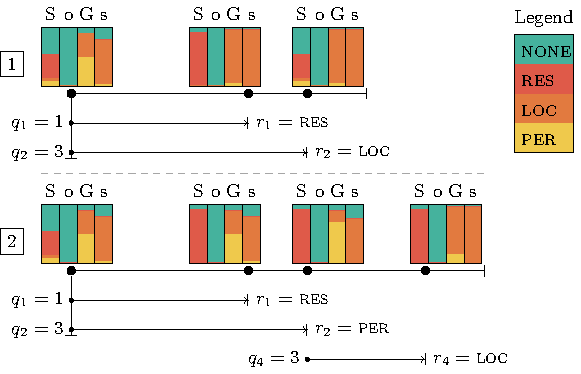
\includegraphics[width=\textwidth]{figures/behavior.pdf}
      \caption{
      {\bf Incorporating information from responses.}
      The bar graphs represent the marginals over the labels for each token (indicated by the first character) at different points in time. 
      The two timelines show how the system updates its confidence over labels based on the crowd's responses.
      The system continues to issue queries until it has sufficient confidence on its labels. 
      See the paragraph on behavior in \sectionref{model} for more information.
      }
\label{fig:behavior}
    \end{subfigure}
    \hfill
    \begin{subfigure}[b]{0.38\textwidth}
%      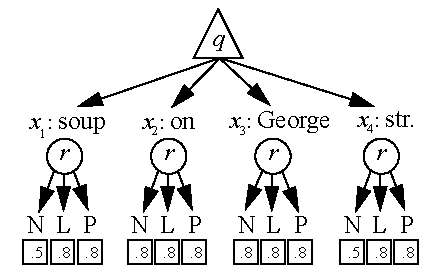
\includegraphics[width=\textwidth,height=0.23\textheight,keepaspectratio]{figures/single-move.pdf}\\[1.7ex]
      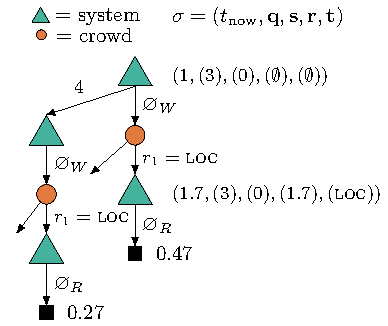
\includegraphics[width=\textwidth,height=0.23\textheight,keepaspectratio]{figures/mcts_simple.pdf}\\[1.7ex]
      \caption{
      {\bf Game tree.} An example of a partial game tree constructed by the system when deciding which action to take in the state $\sigma = (1, (3), (0), (\emptyset), (\emptyset))$, i.e.\ the query $q_1 = 3$ has already been issued and the system must decide whether to issue another query or wait for a response to $q_1$.
      }
\label{fig:tree}
    \end{subfigure}
  \end{centering}
\caption{Example behavior while running structure prediction on the tweet ``Soup on George str.''
We omit the \scres{} from the game tree for visual clarity.
}
\label{fig:game-tree}
\end{figure}


% ARUN: This is a little too much detail too early.  
% Define game top-down
% We define a stochastic game with two players, the system and the crowd.
% The system gets ``woken up'' every time something in the environment changes, and is allowed to make a move.
% The game starts with a $\bx$ arriving in need of a label, and the system must make a decision.
% Possible decisions are TURN\_IN, WAIT, and launching a query $q_0$ on one of the variables $\by_i$.
% If the system decides to TURN\_IN, the best guess $P_{\theta}(\bx|\by)$


% High-level what is the game?
We model on-the-job learning as a stochastic game with two players: the system and the crowd.
The game starts with the system receiving input $\bx$ and ends when the system turns in a set of labels $\by = (y_1, \ldots, y_n)$. 
During the system's turn, the system may choose a query action $q \in \{1, \ldots, n\}$ to ask the crowd to label $y_q$. 
The system may also choose 
the wait action ($q = \acwait$) to wait for the crowd to respond to a pending query
or
the return action ($q = \acret$) to terminate the game and return its prediction given responses received thus far.
%\footnote{When $q = \acwait$ or $q = \acret$, $y_q$ is not defined and is ignored.}
The system can make as many queries in a row (i.e.\ simultaneously) as it wants, before deciding to wait or turn in.\footnote{
This rules out the possibility
of launching a query midway through waiting for the next response. However, we
feel like this is a reasonable limitation that significantly simplifies the
search space.
}
When the wait action is chosen, the turn switches to the crowd, which provides a response $r$ to one pending query, and advances the game clock by the time taken for the crowd to respond.
The turn then immediately reverts back to the system.
When the game ends (the system chooses the return action), the system evaluates a utility that depends on the accuracy of its prediction,
the number of queries issued and the total time taken.
The system should choose query and wait actions to
maximize the utility of the prediction eventually returned.

In the rest of this section, we describe the details of the game tree, our choice of utility and specify models for crowd responses, followed by a brief exploration of behavior admitted by our model.
%The key challenge is to determine which actions the system should take to maximize its expected utility at the end of the game.

\paragraph{Game tree.}
Let us now formalize the game tree in terms of its states, actions, transitions and rewards; see \figureref{tree} for an example. 
The \emph{game state} $\sigma = (\now, \bq, \bs, \br, \bt)$
consists of the current time $\now$, the actions $\bq = (q_1, \ldots, q_{k-1})$ that have been issued at times $\bs = (s_1, \ldots, s_{k-1})$ and
the responses $\br = (r_1, \ldots, r_{k-1})$ that have been received at times $\bt = (t_1, \ldots, t_{k-1})$.
Let $r_j = \emptyset$ and $t_j = \emptyset$ iff
$q_j$ is not a query action or
its responses have not been received by time $\now$.
%Note that some or all of $\br[\now]$ may be $\emptyset$ because those responses have not yet been received.

During the system's turn,
%we query a position $q_k \in \{1, \dots, n\}$ (not necessarily new),
%wait for a response ($q_k = \acwait$) or return the best answer incorporating the responses received thus far ($q_k = \acret$).
when the system chooses an action $q_k$,
the state is updated to $\sigma' = (\now, \bq', \bs', \br', \bt')$, where $\bq' = (q_1, \ldots, q_k)$, $\bs' = (s_1, \ldots, s_{k-1}, \now)$, $\br' = (r_1, \ldots, r_{k-1}, \emptyset)$ and $\bt' = (t_1, \ldots, t_{k-1}, \emptyset)$.
If $q_k \in \{1, \ldots n\}$, then the system chooses another action from the new state $\sigma'$.
If $q_k = \acwait$, the crowd makes a stochastic move from $\sigma'$.
Finally, if $q_k = \acret$, the game ends, and the system returns its best estimate of the labels using the responses it has received and
%$\hat\by \eqdef \argmax_{\by} p(\by \given \bx, \br)$,
obtains a utility $U(\sigma)$ (defined later).
%Both the prediction model $p(\by \given \bx, \br)$ and the utility $U(\sigma)$ will be defined below.

Let $F = \{1 \le j \le k-1 \given q_j \neq \acwait \wedge r_j = \emptyset \}$ be the set of \emph{in-flight} requests.
During the crowd's turn (i.e.\ after the system chooses $\acwait$), the next response from the crowd, $j^* \in F$, is chosen: $j^* = \argmin_{j \in F} t'_j$ where $t'_j$ is sampled from the \emph{response-time model}, $t'_j \sim \ptime(t'_j \given s_j, t'_j > \now)$, for each $j \in F$. Finally, a response is sampled using a response model, $r'_{j^*} \sim p(r'_{j^*} \given \bx, \br)$, and the state is updated to $\sigma' = (t_{j^*}, \bq, \bs, \br', \bt')$, where $\br' = (r_1, \ldots, r'_{j^*}, \ldots, r_k)$ and $\bt' = (t_1, \ldots, t'_{j^*}, \ldots, t_k)$.

\paragraph{Utility.}
% Utility.
% How is the game played? maximizing utility under the model, which will be subsequently.
Under Bayesian decision theory, the \emph{optimal choice} for an action in state $\sigma = (\now, \bq, \br, \bs, \bt)$ is the one that attains the maximum expected utility (i.e.\ value) for the game starting at $\sigma$.
Recall that the system can return at any time, at which point it receives a utility
that trades off two things:
The first is the accuracy of the MAP estimate according to the model's best guess of $\by$ incorporating all responses received by time $\tau$.
The second is the cost of making queries: a (monetary) cost $\weightmoney$ per query made and penalty of $\weighttime$ per unit of time taken.
Formally, we define the utility to be:
\begin{align}
  \label{eqn:utility}
  U(\sigma) &\eqdef \text{ExpAcc}(p(\by \given \bx, \bq, \bs, \br, \bt)) - (n_\text{Q} \weightmoney + \now \weighttime), \\
  \text{ExpAcc}(p) &= \E_{p(\by)}[\text{Accuracy}(\arg\max_{\by'} p(\by'))],
\end{align}
where $n_\text{Q} = |\{j \given q_j \in \{1, \ldots, n\}|$ is the number of queries made,
$p(\by \given \bx, \bq, \bs, \br, \bt)$ is a prediction model that incorporates the crowd's responses.

The utility of wait and return actions is computed by taking expectations over subsequent trajectories in the game tree. 
This is intractable to compute exactly, so we propose an approximate algorithm in \sectionref{game-playing}.

%\equationref{utility} is related to \equationref{value} by considering the utility at the time of the last request, $\tmax = \max\{t_1, \ldots, t_k\}$: $U(\bq, \bs, \br) = \E_{\bt}[U_{\tmax}(\bq, \bs, \br, \bt)]$.
%In practice, we actually consider the utility at the earlier of $\tmax$ and a specified time limit to respond, $\deadline$.
%
%
%\begin{align}
%  \label{eqn:value}
%V^* = \max_{\bq} \E_{p(\br \mid \bx, \bq)}[U(\bq, \br)],
%\end{align}
%where $\br = (r_1, \ldots, r_k)$ are the responses to the queries, $p(\br \mid \bx, \bq)$ is the system's model of the environment and $U(\bq, \br)$ is the utility which captures the cost of making the queries and the accuracy of the predictions given the responses. 
%We will define these latter two quantities next.

%We will define these latter two quantities after looking at the example below:

%The \emph{value} of the game is the maximum expected utility:
%\begin{align}
%  V^* = \max_q \E_{p(r \mid \bx, q)}[U(q, r)],
%\end{align}
%and the \emph{optimal policy} is to choose the action $q$ that attains $V^*$.


% Arun: I don't think this is very useful -V
%Note that the system computes the $V^*$ by only \emph{simulating} possible futures, not by actually querying the crowd.

% Example time!
%Let us look at the example in \figureref{game-tree} more intuitively:
%querying one of the end positions ($q = 1$ or $q = 4$),
%is less informative than choosing the middle positions ($q = 2$ or $q = 3$),
%assuming the model propagates information between adjacent positions.
%Indeed, the expected utilities with a uniform distribution over $r$
%are $0.7$, $0.8$, $0.8$, and $0.7$, respectively, and so both $q = 2$ and $q = 3$ are optimal actions.

%Note that the system computes the $V^*$ by only \emph{simulating} possible futures, not actually querying the crowd.
%The simulation is based on the transition probabilities $p(r \mid \bx, q)$ and the utilities $U(q, r)$, which are based on a probabilistic model that connects input, output, responses, and time delays.

% Start model.
\paragraph{Environment model.}

The final component is a model of the environment (crowd).
Given input $\bx$ and queries $\bq = (q_1, \dots, q_k)$ issued at times $\bs = (s_1, \dots, s_k)$,
we define a distribution over the output $\by$, responses $\br = (r_1, \dots, r_k)$
and response times $\bt = (t_1, \dots, t_k)$ as follows:
\begin{align}
  \label{eqn:dynamics}
%p(\by, \br, \bt \mid \bx, \bq) \eqdef \p(\by \given \bx) \prod_{i=1}^k \presp(r_i \mid \bx, \by, q_i) \ptime(t_i \mid \bx, \by, q_i, s_i).
p(\by, \br, \bt \given \bx, \bq, \bs) \eqdef \p(\by \given \bx) \prod_{i=1}^k \presp(r_i \mid y_{q_i}) \ptime(t_i \mid s_i).
\end{align}
The three components are as follows:
$\p(\by \given \bx)$ is the \emph{prediction model} (e.g.\ a standard linear-chain CRF);
$\presp(r \given y_q)$ is the \emph{response model} which describes the
distribution of the crowd's response $r$ for a given a query $q$ when the true
answer is $y_q$;
and $\ptime(t_i \mid s_i)$ specifies the latency of query $q_i$.
%\footnote{Of course, $\ptime$ and $\presp$ can easily be extended to depend arbitrarily on the input $\bx$.} 
%If the crowd workers were infallible we could define $\presp(r \given y_q)$ to
The CRF model $\p(\by \given \bx)$ is learned based on all actual responses
(not simulated ones) using AdaGrad.
To model annotation errors, we set $\presp(r \given y_q)
= 0.7$ iff $r = y_q$,\footnote{We found the humans we hired were roughly 70\%
accurate in our experiments} and distribute the remaining probability for $r$
uniformly.
%
% Finally, $\ptime(t \given s)$ is the \emph{time delay model}, which governs how long a given query $q$ will take. While, in reality, $t$ depends on many factors including the input, in the interest of simplicity we assume $t - s$ to be drawn from a gamma distribution with globally fixed parameters.We also define the \emph{response at time $\tau$}, $r[\tau]$, to be $r$ if $\tau > t$ and $\emptyset$ otherwise.
%
% Doing things with the model
Given this full model, we can compute $p(r' \mid \bx, \br, q)$ simply by marginalizing out $\by$ and $\bt$ from \equationref{dynamics}.
When conditioning on $\br$, we ignore responses that have not yet been received (i.e.\ when $r_j = \emptyset$ for some $j$).
%Given this full model, we can compute $p(\br \mid \bx, \bq)$ simply by marginalizing out $\by$ and $\bt$ from \equationref{dynamics}.
%We can also compute the distribution over responses at a particular time $\tau$, $p(\br[\tau] \given \bx, \bq)$, where $\br[\tau] = (r_1[\tau], \ldots, r_k[\tau])$.
% Describe the simplifications on how time is moved forward, with possibly an example

%Importantly, we are only conditioning on the responses $\br[t]$ that are available at time $t$.

% Behavior!
\paragraph{Behavior.}
Let's look at typical behavior that we expect the model and utility to capture.
\figureref{behavior} shows how the marginals over the labels change as the crowd provides responses for our running example, i.e.\ named entity recognition for the sentence ``Soup on George str.''.
In the both timelines, the system issues queries on ``Soup'' and ``George'' because it is not confident about its predictions for these tokens.
In the first timeline, the crowd correctly responds that ``Soup'' is a resource and that ``George'' is a location.
Integrating these responses, the system is also more confident about its prediction on ``str.'', and turns in the correct sequence of labels.
In the second timeline, a crowd worker makes an error and labels ``George'' to be a person.
The system still has uncertainty on ``George'' and issues an additional query which receives a correct response, following which the system turns in the correct sequence of labels.
While the answer is still correct, the system could have taken less time to respond by making an additional query on ``George'' at the very beginning.

%Secondly, we expect the system to use queries judiciously when the cost per query, $\weightmoney$, is significant compared to the cost per unit time, $\weighttime$.
%Continuing with the previous example, when $\weightmoney = $ and $\weighttime = $, the system will prefer to wait for a response for the token ``George'' before asking a label for ``str.''.
%However, it will simultaneously ask for a label for ``Soup'' because the response from ``George'' is unlikely to affect the prediction for ``Soup''.


%Firstly, because the system wants to maximize the accuracy while minimizing the number of queries, it will prioritize asking queries that provide the most information.
%For example,
%in \figureref{game-tree}, getting the crowd to label on the token ``George'' provides information not only to its label, but also to the adjacent token ``str.''. Hence, the system prioritizes asking ``George'' over asking for ``str.''. %\todo{Update figure, and have actual numbers here.}

%in the model in \figureref{game-tree}, the model, a linear-chain CRF, propagates information between adjacent labels. 
%Thus, querying one of the middle positions ($q = 2$ or $q = 3$) can be more informative than one of the end positions ($q = 1$ or $q = 4$).
%Indeed, this is reflected in the expected utilities of each query: with a uniform distribution over the responses, they are $0.7$, $0.8$, $0.8$, and $0.7$ respectively. Thus, both $q = 2$ and $q = 3$ are optimal actions. \todo{This is a really lame example with poor intuition.}

%Secondly, we expect the system to use queries judiciously when the cost per query, $\weightmoney$, is significant compared to the cost per unit time, $\weighttime$.
%Continuing with the previous example, when $\weightmoney = $ and $\weighttime = $, the system will prefer to wait for a response for the token ``George'' before asking a label for ``str.''.
%However, it will simultaneously ask for a label for ``Soup'' because the response from ``George'' is unlikely to affect the prediction for ``Soup''.
%\todo{make this happen!}

%\todo{Figurewise, we should have a figure that shows the change in probabilities of labels down the tree.}

%If we had already made one query $q_1$ and gotten a response $r_1$,
%we can incorporate the evidence, which will propagate through the CRF
%and inform the distribution over possible responses $r_2$ for the next query $q_2$:
%$p(r_2 \mid \bx, q_1, r_1, q_2)$.
%
%\todo{WEIRD}
%The temporal aspect of the model also allows for interesting possibilities
%and is important for handling asynchronous queries and responses.
%Suppose we made a query $q_1$ at time $s_1$ but have not yet gotten response $r_1$.
%We might still want to ask for various probabilities \emph{at time} $t$,
%which involves integrating over possible future responses $r_1$ and response times $t_1$.
%Formally, define $r_i[t]$ to be the response at time $t$, which is equal to $r_i$ if $t_i \le t$
%or $\emptyset$ if $t_i > t$.
%Then we could ask about the probability of a response $r_2$ at time $t$,
%which integrates over the possibility of having received $r_1$ or not:
%\begin{align}
%p(r_2[t] \mid \bx, q_1, q_2) = p(t_1 \le t \mid s_1) p(r_2[t] \mid \bx, q_1, r_1, q_2) + p(t_1 > t \mid s_1) p(r_2[t] \mid \bx, q_2).
%\end{align}
%
%Let us revisit the example in \figureref{game-tree} by looking at the game tree on the right where the system turns in an answer after a single query.
%The square leaf nodes store the value of obtaining responses for each query.
%Intuitively, because the model (a linear-chain CRF) propagates information between adjacent labels, querying one of the end positions ($q = 1$ or $q = 4$) is less informative than the middle positions ($q = 2$ or $q = 3$).
%Indeed, this is reflected in the expected utilities of each query: with a uniform distribution over the responses, they are $0.7$, $0.8$, $0.8$, and $0.7$ respectively. Thus, both $q = 2$ and $q = 3$ are optimal actions.
%\todo{this is a bit of a lame example.}

